\chapter{\texorpdfstring{Robustezza alle incertezze: analisi e sintesi con $\mu$}{Robustezza alle incertezze: analisi e sintesi con mu}}
\label{cap:mu}
\section{Dalle prove nominali alle incertezze fisiche}
Le prove del capitolo precedente descrivono il comportamento del
controllore sul modello nominale. A questo punto vogliamo capire
che cosa succede quando i parametri reali del manipolatore differiscono
 dai valori nominali. Una rigidezza diversa sposta le risonanze SEA;
un'inerzia motore diversa modifica la dinamica interna; una dinamica
attuativa non modellata può alterare modulo e fase del feedback.

La domanda non è più se un singolo modello risponde bene, ma se
il sistema rimane stabile e rispetta la prestazione pesata per
\emph{tutta} la famiglia ammessa. Confrontiamo il controllore
$H_\infty$ 2-DoF e $K_\mu$ mantenendo gli stessi $W_e,W_u,M_o$,
lo stesso disturbo lato link e la stessa mappa $[r;d]\mapsto[z_e;z_u]$.
Le incertezze sono quelle del Capitolo 5, dichiarate prima della sintesi.

\subsection{I tre parametri meccanici selezionati}
Sono incerti $k_1,k_2$ e $J_{m1}$, indipendenti e reali.
Le rigidezze possono variare per materiali e assemblaggio; l'inerzia
riflessa del primo motore dipende anche dalla modellazione
 dell'azionamento. Il 10\% è un'ipotesi ingegneristica del progetto,
non una tolleranza misurata né un intervallo statistico.

\begin{table}[htbp]\centering\small
\begin{tabular}{lrrl}\toprule
Parametro & Nominale & Intervallo & Oggetto MATLAB\\\midrule
$k_1$ [N m/rad] & 50 & $[45,55]$ & \texttt{ureal('k1',50,\ldots)}\\
$k_2$ [N m/rad] & 40 & $[36,44]$ & \texttt{ureal('k2',40,\ldots)}\\
$J_{m1}$ [kg m$^2$] & 0.01 & $[0.009,0.011]$ & \texttt{ureal('Jm1',0.01,\ldots)}\\\bottomrule
\end{tabular}
\caption{I tre scalari reali usano \texttt{'Percentage',10},
come definito nella funzione centrale dei parametri incerti.}
\end{table}
Masse, geometrie, $J_{m2}$, attriti e gravità restano nominali.
È una scelta per contenere il numero di parametri incerti,
non una dichiarazione che siano fisicamente esatti.

\subsection{La dinamica degli attuatori}
Per costruire la famiglia attuativa si variano frequenza naturale,
smorzamento e ritardo. Le prime due influenzano rapidità e risonanza;
il ritardo include dispersioni di latenza e jitter.

\begin{table}[htbp]\centering
\begin{tabular}{lrrr}\toprule
Grandezza & Nominale & Variazione & Intervallo\\\midrule
$\omega_n$ [rad/s] & 40 & $\pm10\%$ & $[36,44]$\\
$\zeta$ & 0.8 & $\pm10\%$ & $[0.72,0.88]$\\
Ritardo [ms] & 15 & $\pm20\%$ & $[12,18]$\\\bottomrule
\end{tabular}
\caption{Intervalli usati per costruire l'inviluppo degli errori
attuativi; non sono tre ulteriori blocchi \texttt{ureal} nella pianta finale.}
\end{table}
La famiglia contiene 120 attuatori: nominale, sei variazioni singole,
otto vertici e 105 campioni riproducibili. L'errore relativo rispetto
all'attuatore nominale è raccolto nell'inviluppo
\[
 W_I(s)=\frac{2.929983729s+3.748469010}{s+206.973575453}.
\]
Il fit usa margine 1.08 e il massimo rapporto campionato
 fra errore relativo e inviluppo è 0.92593. Questa verifica
copre i campioni costruiti, non ogni possibile attuatore fisico.
La rappresentazione finale per ciascun canale è
\[
 G_{ai}^{\Delta}=G_{a0}(1+W_I\Delta_{ai}),\qquad
 \|\Delta_{ai}\|_\infty\le1,\quad i=1,2.
\]
$\Delta_{ai}$ è una dinamica scalare stabile ignota, rappresentata
con \texttt{ultidyn}. I due canali sono indipendenti.
Nell'analisi robusta si considera tutto questo insieme matematico,
più ampio della sola lista di attuatori usata per il fit.

\section{Raccogliere le incertezze in \texorpdfstring{$\Delta$}{Delta}}
Per passare dalle grandezze fisiche a una rappresentazione comune,
esprimiamo i parametri come scostamenti normalizzati. Per esempio
\[
 k_1=50(1+0.1\delta_{k1}),\qquad \delta_{k1}\in[-1,1].
\]
$\delta_{k1}=0$ è il nominale; $\delta_{k1}=1$ dà 55 N m/rad.
La stessa idea vale per $k_2$ e $J_{m1}$. La normalizzazione
non cambia gli intervalli: rende la soglia uno comune ai blocchi.
Le dipendenze fisiche, incluso l'inverso di $J_{m1}$, sono
conservate nel modello; non si aggiunge un errore arbitrario ad $A$.

MATLAB estrae la struttura
\begin{equation}\label{eq:deltafive}
 \Delta=\operatorname{diag}(\Delta_{a1},\Delta_{a2},
 \delta_J,\delta_{k1},\delta_{k2})\in\mathbb C^{5\times5}.
\end{equation}
I primi due blocchi sono dinamici scalari complessi, gli ultimi tre
scalari reali. Il campo \texttt{Occurrences} vale uno per ciascuno
 dei cinque blocchi nella rappresentazione salvata. Non si conta
il numero di blocchi dal numero di apparizioni del simbolo nelle
 equazioni. Le due dinamiche non sono fuse in un blocco pieno
$2\times2$, che ammetterebbe accoppiamenti diversi da quelli scelti.

\section{Separare la parte nota: lo schema \texorpdfstring{$N$--$\Delta$}{N--Delta}}
Fissiamo prima il controllore. Possiamo poi vedere il sistema
chiuso come due parti collegate: $N$ contiene ciò che conosciamo,
compresi il controllore e i pesi; $\Delta$ contiene gli scostamenti
ammessi. $N$ manda il segnale $v_\Delta$ alla parte incerta e ne
riceve $w_\Delta=\Delta v_\Delta$. Questa è la rappresentazione
$N$--$\Delta$ mostrata in Figura~\ref{fig:ndelta}.

\begin{figure}[htbp]\centering
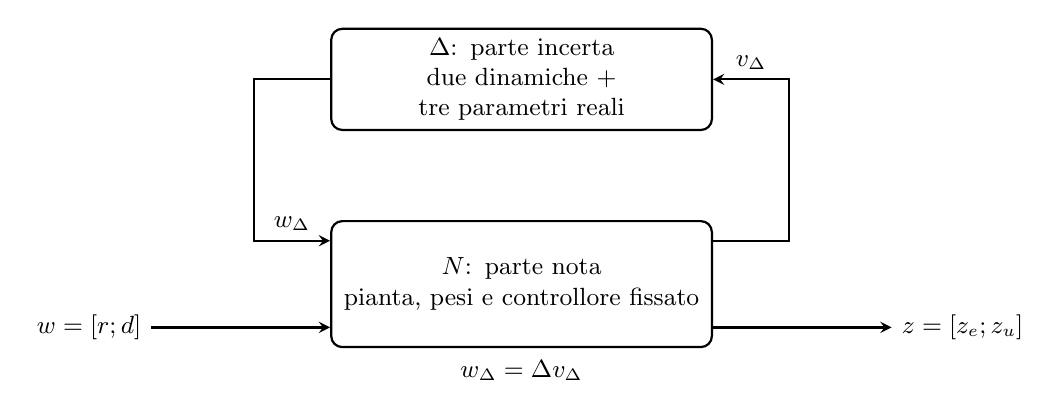
\begin{tikzpicture}[>=stealth,thick,
 b/.style={draw,rounded corners,align=center,text width=4.6cm},
 every node/.style={font=\small}]
\node[b,minimum height=1.6cm] (n) at (0,0)
 {$N$: parte nota\\pianta, pesi e controllore fissato};
\node[b,minimum height=1.2cm] (d) at (0,2.6)
 {$\Delta$: parte incerta\\due dinamiche + tre parametri reali};
\draw[->] (n.east |- 0,.55) -- (3.4,.55) -- (3.4,2.6)
 -- node[above] {$v_\Delta$} (d.east);
\draw[->] (d.west) -- (-3.4,2.6) -- (-3.4,.55)
 -- node[above] {$w_\Delta$} (n.west |- 0,.55);
\draw[->] (-4.7,-.55) node[left] {$w=[r;d]$} -- (n.west |- 0,-.55);
\draw[->] (n.east |- 0,-.55) -- (4.7,-.55) node[right] {$z=[z_e;z_u]$};
\node at (0,-1.1) {$w_\Delta=\Delta v_\Delta$};
\end{tikzpicture}

\caption{A controllore fissato, $N$ raccoglie la parte nota e
$\Delta$ i cinque blocchi incerti. $w=[r;d]$ e $z=[z_e;z_u]$
conservano il significato del Capitolo 8.}\label{fig:ndelta}
\end{figure}
Solo dopo aver distinto le due parti scriviamo le loro connessioni:
\[
 \begin{bmatrix}v_\Delta\\z\end{bmatrix}
 =\begin{bmatrix}N_{11}&N_{12}\\N_{21}&N_{22}\end{bmatrix}
 \begin{bmatrix}w_\Delta\\w\end{bmatrix},\qquad
 w_\Delta=\Delta v_\Delta.
\]
$N_{11}$ è il ritorno fra le porte dell'incertezza;
$N_{22}$ è la mappa nominale esterna quando $\Delta=0$.
Nel nostro caso $N$ è $9\times9$, con cinque canali interni
 e quattro ingressi esterni/uscite pesate. Quindi $N_{11}$
è $5\times5$ e $N_{22}$ è $4\times4$.

La LFT è il modo compatto di indicare questa connessione.
La chiusura di $K$ su $P_\Delta$ è una LFT inferiore;
la separazione di $\Delta$ da $N$ è una LFT superiore.
Nel codice la matrice chiamata $N$ nel testo è \texttt{M}:
\begin{lstlisting}
CL=lft(P,K);
[M,Delta,BlkStruct,NormUnc]=lftdata(CL);
CLcheck=lft(Delta,M);
\end{lstlisting}
La terza riga ricompone il modello nella convenzione MATLAB.
Non va invertito l'ordine degli argomenti mantenendo la stessa
partizione. La ricostruzione nominale è stata verificata; le
formule complete sono nell'Appendice~\ref{app:matlab}.

\section{Che cosa misura \texorpdfstring{$\mu$}{mu}}
$\mu$ aiuta a capire quanto la struttura d'incertezza ammessa è
vicina a causare una condizione critica. Si cerca la più piccola
perturbazione, con gli stessi tipi di blocchi, capace di rendere
singolare il ritorno interno $I-N_{11}\Delta$. $\mu$ è l'inverso
 della sua grandezza.

Se il picco di $\mu$ è minore di uno, la condizione critica
richiede un'incertezza più grande di quella normalizzata ammessa,
con le usuali ipotesi di stabilità nominale e buona posizione
 dell'interconnessione. Se supera uno, la robusta stabilità
può venire meno già entro il dominio dichiarato.
Non è una probabilità di guasto: tiene conto della struttura,
non di una distribuzione statistica delle incertezze.

Il calcolo esatto è difficile, quindi si usano due limiti
$\underline\mu\le\mu\le\overline\mu$.
La maggiorazione serve a escludere una criticità nel dominio;
la minorazione deriva dalla ricerca di perturbazioni critiche.
Se i limiti non permettono una decisione rispetto alla soglia
uno, il risultato rimane inconclusivo. Scaling D, e anche G
per i blocchi reali, servono a calcolare queste maggiorazioni.
Il loro dettaglio numerico non modifica il significato fisico
 dei cinque blocchi.

\section{Prestazione nominale, stabilità e prestazione robuste}
\subsection{Prima il caso nominale: NS e NP}
NS richiede stabilità interna per $\Delta=0$.
NP aggiunge $\|T_{zw,0}\|_\infty<1$.
La stabilità è controllata prima della norma, sulla realizzazione
completa. NP non equivale a rispettare tutti i target temporali:
il capitolo precedente ha mostrato un $H_\infty$ con NP positiva
 e assestamento oltre 0.8 s.

\subsection{Stabilità robusta: RS}
RS chiede stabilità per tutte le incertezze ammesse.
Si studia il ritorno $N_{11}$ con la struttura fisica $\Delta$.
Il margine $m_{RS}$ dice di quanto si possono amplificare insieme
 gli scostamenti normalizzati prima della condizione critica.
Per esempio, un margine maggiore di uno copre il dominio scelto;
un margine minore di uno indica che esso è troppo ampio per il
controllore considerato.

Il codice corrente usa \texttt{robstab}, che restituisce limiti
 inferiore e superiore del margine. Se il limite inferiore supera
uno, RS è soddisfatta nel modello; se quello superiore è sotto
uno, RS è esclusa. Se l'intervallo attraversa uno, non si accredita
la proprietà. I margini non sono valori di $\mu$.

\subsection{Prestazione robusta: RP}
RP richiede stabilità e $\|T_{zw}(\Delta)\|_\infty<1$ per tutta
la famiglia. Un sistema può quindi essere robustamente stabile
 ma non rispettare le prestazioni pesate.
Per interpretare RP si può aggiungere un blocco fittizio di
prestazione che richiude $z$ su $w$. Nel nostro problema è un
blocco complesso pieno $\Delta_p$ di dimensione $4\times4$:
non è un nuovo parametro fisico del robot.

\begin{figure}[htbp]\centering
\resizebox{.8\textwidth}{!}{\providecommand{\SeaDeltaLabel}{cinque blocchi fisici}
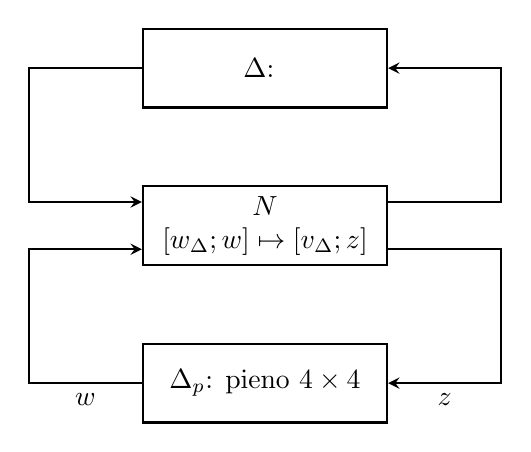
\begin{tikzpicture}[>=stealth,thick,b/.style={draw,align=center,minimum height=1cm,minimum width=3.1cm}]
\node[b] (n) at (0,0) {$N$\\$[w_\Delta;w]\mapsto[v_\Delta;z]$};
\node[b] (d) at (0,2) {$\Delta$: \SeaDeltaLabel};
\node[b] (p) at (0,-2) {$\Delta_p$: pieno $4\times4$};
\draw[->] (n.east |- 0,.3)--(3,.3)--(3,2)--(d.east);
\draw[->] (d.west)--(-3,2)--(-3,.3)--(n.west |- 0,.3);
\draw[->] (n.east |- 0,-.3)--(3,-.3)--(3,-2)--node[below]{$z$}(p.east);
\draw[->] (p.west)--node[below]{$w$}(-3,-2)--(-3,-.3)--(n.west |- 0,-.3);
\end{tikzpicture}
}
\caption{Interpretazione di RP con il blocco fittizio $\Delta_p$.
Le incertezze fisiche conservano la loro struttura.}
\end{figure}
Nel percorso finale si usa \texttt{robgain(CL,1)}: scala le
incertezze fisiche lasciando fissata la soglia prestazionale uno.
Questo margine non è semplicemente l'inverso della norma nominale.
Le chiamate effettive in \path{run_hinf_final_robust.m} sono
\begin{lstlisting}
[a.RS,a.rsWorst,a.rsInfo]=robstab(a.CL);
[a.RP,a.rpWorst,a.rpInfo]=robgain(a.CL,1);
\end{lstlisting}
I nomi \texttt{robuststab} e \texttt{robustperf} non sono usati
nelle chiamate del repository: il progetto impiega \texttt{robstab}
e \texttt{robgain}. Esiste inoltre un calcolo diretto di
\texttt{mussv} su griglia nelle analisi precedenti. L'appendice
lo mostra come esempio della procedura storica, senza trasferirne
i numeri ai controllori finali.

\subsection{Esito del controllore nominale}
Il controllore $H_\infty$ di ordine \FinalOrder\ supera NS e NP,
ma il margine RS è
\[
 m_{RS}\in[\FinalHRSLowerBound,\FinalHRSUpperBound],
 \qquad\omega_{\rm crit}\simeq70.32\ \mathrm{rad/s}.
\]
Entrambi gli estremi sono molto minori di uno. La frequenza è
vicina ai modi elastici: suggerisce una compensazione nominale
fragile in quella zona, senza identificare da sola un parametro
responsabile. L'intervallo RP restituito è invece invertito,
circa $[0.0172543,0.0171945]$, anche dopo la ricerca rinforzata
\texttt{MussvOptions='m9'}. Non ne scambiamo gli estremi:
la stima numerica del margine RP è non validata. RP è comunque
esclusa dal fallimento RS, che è una sua condizione necessaria.

\section{Progettare per le incertezze: \texorpdfstring{$\mu$-synthesis}{mu-synthesis}}
Finora abbiamo analizzato un controllore progettato sul nominale.
La $\mu$-synthesis considera invece le incertezze durante la
sintesi. Nel progetto si usa \texttt{musyn}, con iterazione D--K:
\begin{enumerate}
\item si ottiene un controllore per il problema scalato iniziale;
\item con il controllore fissato si valuta dove l'incertezza è più critica;
\item si aggiornano gli scaling che descrivono il peso delle direzioni critiche;
\item si approssimano gli scaling con trasferimenti razionali;
\item si risintetizza un controllore $H_\infty$ per la pianta scalata;
\item si ripete fino al criterio di arresto o al numero massimo di iterazioni.
\end{enumerate}
Con blocchi reali e dinamici si usano scaling D/G; D--K è il
nome usuale del procedimento. L'alternanza non dimostra un
ottimo globale. Le dinamiche del fit possono aumentare
l'ordine del controllore.

\begin{figure}[htbp]\centering
\resizebox{.94\textwidth}{!}{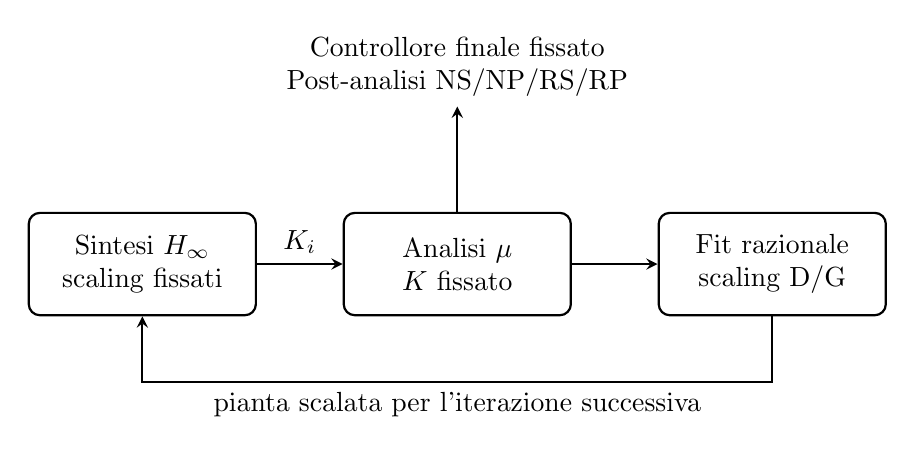
\begin{tikzpicture}[>=stealth,thick,b/.style={draw,rounded corners,align=center,text width=2.65cm,minimum height=1.3cm}]
\node[b] (k) at (0,0) {Sintesi $H_\infty$\\scaling fissati};
\node[b] (m) at (4,0) {Analisi $\mu$\\$K$ fissato};
\node[b] (f) at (8,0) {Fit razionale\\scaling D/G};
\draw[->] (k)--node[above]{$K_i$}(m);\draw[->] (m)--(f);
\draw[->] (f.south)--(8,-1.5)--node[below]{pianta scalata per l'iterazione successiva}(0,-1.5)--(k.south);
\draw[->] (m.north)--(4,2)node[above,align=center]{Controllore finale fissato\\Post-analisi NS/NP/RS/RP};
\end{tikzpicture}
}
\caption{Iterazione di sintesi. Alla fine il controllore viene
fissato e analizzato sulla pianta incerta originale.}
\end{figure}
La chiamata reale è
\begin{lstlisting}
[K,objective,info]=musyn(P,4,2,opts);
\end{lstlisting}
$P$ è qui la pianta generalizzata incerta 2-DoF; rimangono quattro
segnali $[r;q]$ per il controllore e due comandi.
È stata eseguita una campagna di cinque iterazioni, con
\texttt{MixedMU='on'}, scaling D/G e griglia di 1201 frequenze
fra $10^{-3}$ e $10^4$ rad/s. Opzioni e seed sono salvati
insieme al risultato e riassunti nell'Appendice~\ref{app:matlab}.

\begin{figure}[htbp]\centering
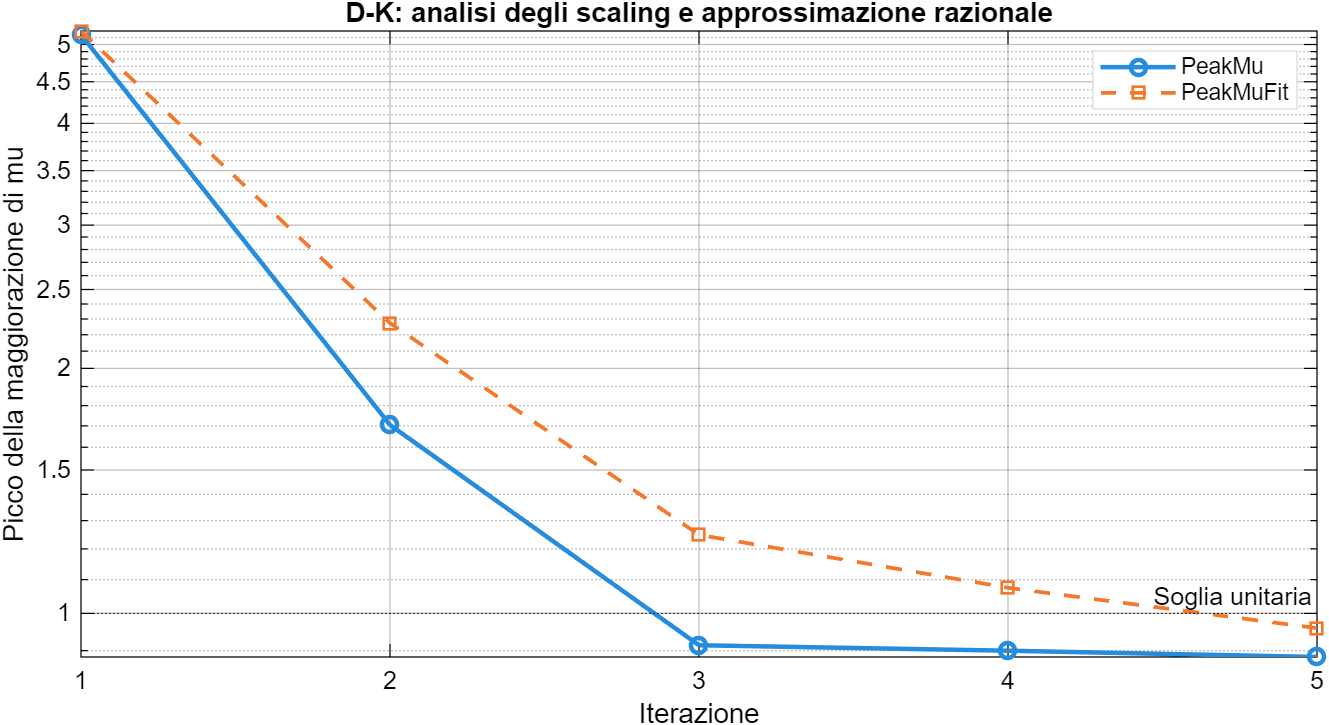
\includegraphics[width=.85\textwidth]{figures/mu/dk_history.png}
\caption{Picchi salvati di $\mu$ e delle rispettive approssimazioni
 dopo il fit. Non sono risultati Monte Carlo.}\label{fig:dkhistory}
\end{figure}
Il picco scende da circa 5.1412 a \FinalMuObjective;
il controllore ottenuto ha ordine \FinalMuOrder.
Il valore finale della sintesi, il picco dopo fit e la norma
nominale sulla pianta originale sono quantità diverse.
Non è stata eseguita una riduzione d'ordine.

\section{Post-analisi e confronto finale di robustezza}
Il controllore salvato viene ricollegato alla stessa pianta
incerta. Si controllano identità del nominale, stabilità interna,
norma e struttura dei blocchi; si ripetono le analisi RS e RP.
I margini non si deducono dal solo obiettivo della sintesi.

\begin{table}[htbp]\centering\small
\begin{tabular}{lcc}\toprule
Quantità & $H_\infty$ 2-DoF & $K_\mu$ 2-DoF\\\midrule
Ordine & \FinalOrder & \FinalMuOrder\\
NS & soddisfatta & soddisfatta\\
Norma nominale & \FinalGamma & \FinalMuGamma\\
NP & soddisfatta & soddisfatta\\
Margine RS & $[\FinalHRSLowerBound,\FinalHRSUpperBound]$ & $[\FinalMuRSLowerBound,\FinalMuRSUpperBound]$\\
Esito RS & non soddisfatta & soddisfatta\\
Margine RP & intervallo non valido & $[\FinalMuRPLowerBound,\FinalMuRPUpperBound]$\\
Esito RP & esclusa da RS & soddisfatta\\
$\omega_{RS}$ [rad/s] & 70.32 & 61.96\\
$\omega_{RP}$ [rad/s] & non accreditata & 9.85\\\bottomrule
\end{tabular}
\caption{Confronto sullo stesso modello incerto e sugli stessi pesi.
Gli intervalli sono limiti del margine.}
\end{table}
\begin{figure}[htbp]\centering
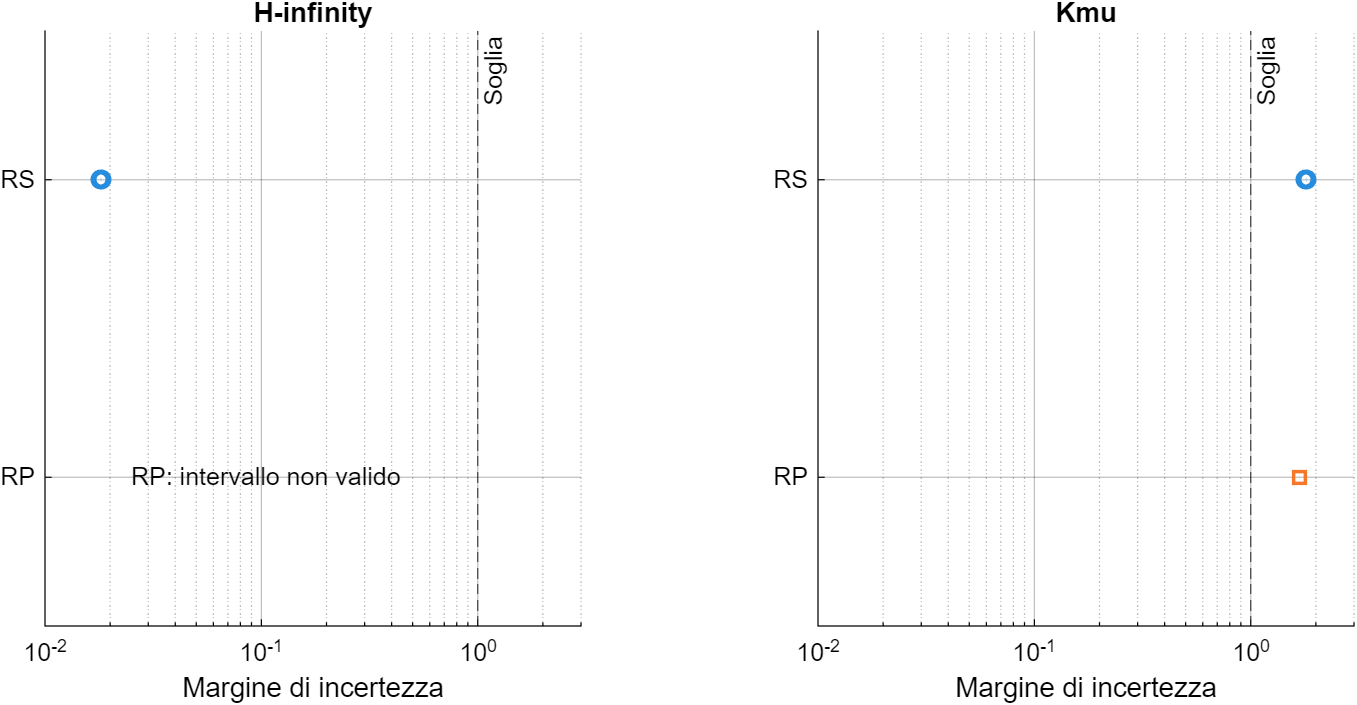
\includegraphics[width=.94\textwidth]{figures/mu/robust_margins.png}
\caption{Margini rispetto alla soglia uno. L'intervallo RP non
valido del controllore nominale non è disegnato come garanzia.}
\end{figure}
Per $K_\mu$ i limiti inferiori RS e RP superano uno: il controllore
soddisfa NS, NP, RS e RP per il modello lineare incerto dichiarato.
La norma nominale \FinalMuGamma\ è peggiore di quella del comparatore
$H_\infty$, ma la proprietà è mantenuta sull'intero dominio modellato.
Il prezzo è l'ordine 78 e un tracking ancora oltre il target:
$T_s=1.522,1.478$ s; sul primo giunto l'errore statico è circa 6\%,
sopra il 5\% richiesto. RP e requisiti temporali sono distinti.

Il campionamento comune conferma empiricamente la differenza:
$H_\infty$ è stabile in 0/40 impianti, $K_\mu$ in 40/40.
I 120 attuatori dell'inviluppo e questi 40 impianti chiusi sono
insiemi usati per scopi diversi. La Monte Carlo non sostituisce
 i margini e non ne dà un'interpretazione probabilistica.
Il dettaglio dei campioni è nel Capitolo 11; le verifiche
non lineari e di rumore nel Capitolo 10 non estendono RS/RP
all'hardware o a fenomeni esclusi dal modello.

\section{Riferimenti per i comandi MATLAB}
Le convenzioni sono documentate da MathWorks per
\href{https://www.mathworks.com/help/robust/ref/inputoutputmodel.lftdata.html}{\texttt{lftdata}},
\href{https://www.mathworks.com/help/robust/ref/dynamicsystem.robstab.html}{\texttt{robstab}},
\href{https://www.mathworks.com/help/robust/ref/dynamicsystem.robgain.html}{\texttt{robgain}}
 e \href{https://www.mathworks.com/help/robust/ug/d-k-iteration-process.html}{iterazione D--K}.
Strutture, numeri e conclusioni derivano dai dati del nostro
repository, tracciati nelle appendici.
